\chapter{Data Foundations and Feature Engineering}
\label{chap:data}

This chapter documents how raw league information is transformed into a unified analytic dataset powering every downstream model. We highlight ingestion flows, schema design, data quality controls, and feature generation strategies that balance expressiveness with reproducibility.



\section{Source Systems and Ingestion}
\begin{itemize}
  \item \textbf{Play-by-play:} nflverse and team-operated feeds provide event-level context including personnel, formation, and tracking-derived metrics.
  \item \textbf{Odds history:} The Odds API snapshots populate the \texttt{odds\_history} table with market-implied expectations across books.
  \item \textbf{Weather and travel:} NOAA archives and team schedule metadata add environment, rest, and travel load features.
\end{itemize}
Ingestion pipelines run inside orchestrated containers with idempotent writes. All raw pulls are versioned and stored in S3-compatible object storage for auditability.\mndown{2}{Ingestion \textrightarrow{} staging \textrightarrow{} feature marts (see Section~\ref{sec:schema-mart}).}

\subsection{Injury hazard and return-to-play}\label{subsec:injury-hazard}
Let $T$ be time lost to injury and $X$ covariates (position, age, prior health). A Cox model
$\lambda(t\mid X)=\lambda_0(t)\exp(\beta^\top X)$ yields a survival $S(t\mid X)$ for expected
downtime. Define an availability prior $\pi_t=\Prob(\text{plays at week }t\mid \text{DNP at }t-1)$
from $S$. We translate $\pi_t$ into team strength adjustments by mapping expected snaps to unit
EPA deltas in the feature set.

\subsection{Opponent adjustment with ridge}\label{subsec:opp-ridge}
Given raw feature $x_{i,t}$ for team $i$, week $t$, model
$x_{i,t} = \alpha_i + \delta_{\text{opp}(i,t)} + \varepsilon_{i,t}$. Ridge-penalized least squares
\[
\min_{\alpha,\delta}\sum_{i,t}\!\big(x_{i,t}-\alpha_i-\delta_{\text{opp}(i,t)}\big)^2
+ \lambda\big(\|\alpha\|_2^2+\|\delta\|_2^2\big)
\]
yields shrunken opponent-adjusted $x_{i,t}^\star=x_{i,t}-\hat\delta_{\text{opp}(i,t)}$ with reduced
variance vs naive demeaning.



\subsection{Orchestration and Idempotency}
Nightly tasks run under containerized runners that interact with the local TimescaleDB instance. Each task is idempotent: it checks for existing records by natural keys (game id, bookmaker, timestamp) and upserts only changed rows. Rate limits for external APIs are enforced via token buckets to avoid sampling artifacts.

\section{Relational Schema and Mart Design}\label{sec:schema-mart}
The TimescaleDB instance exposes three logical layers:
\begin{description}
  \item[Staging:] lightly cleaned mirrors of the source feeds for reproducibility checks.
  \item[Core:] conformed tables such as \texttt{games}, \texttt{plays}, \texttt{teams}, and \texttt{odds\_history} with enforced keys and foreign key constraints.
  \item[Mart:] denormalized analytical views (e.g.\ \texttt{mart.team\_epa}, \texttt{mart.game\_summary})\\ optimized for modeling and reporting.
\end{description}
Schema migrations are version-controlled under \texttt{db/}, and every change includes smoke tests that confirm ingest scripts remain idempotent.

\subsection{Timescale Hypertables and Chunking}
Odds and play-by-play tables are hypertables partitioned by time; chunk sizes balance insert speed with query latency. Compression policies retain recent data uncompressed for writes while compressing historical partitions for analytics.

\subsection{Indexing Strategy}
Composite indexes on \texttt{(game\_id, book, market, quoted\_at)} and partial indexes by market type accelerate common joins. BRIN indexes aid range scans over \texttt{quoted\_at} on large horizons. We include covering indexes for the most frequent analytic queries.

\subsection{Identifiers and Keys}
Stable identifiers are essential. We adopt composite keys for markets (game id, book, market type, quote time) and maintain surrogate keys only where necessary for foreign-key fan-out. Historical corrections (schedule changes, rescheduled games) are recorded with validity intervals to support as-of queries.

\section{Feature Engineering Strategy}
We partition features into modular catalogs so experiments can mix and match by hypothesis:
\begin{itemize}
  \item \textbf{Situational:} down, distance, field zone, score differential, and clock states.
  \item \textbf{Team form:} rolling EPA/play, success rate splits, red-zone efficiency, and drive-level pace.
  \item \textbf{Market signals:} line movement velocity, hold, consensus vs rogue book delta.
  \item \textbf{Roster context:} availability projections, positional depth adjustments, rest differentials.
\end{itemize}
Metadata describing feature lineage, update cadence, and owners is tracked in a YAML manifest to support automated documentation.

\subsection{Encoding and Leakage Controls}
Categoricals use target or one-hot encoding depending on cardinality; temporal features are aligned to the decision timestamp with strict as‑of semantics. Any feature depending on post‑decision information is flagged by lineage checks and rejected during training.

\subsection{Temporal Splits and Leakage Controls}
Train/validation/test splits are formed by contiguous time blocks. Features that are not known at decision time (post-game updates, revised injury statuses) are excluded from training sets. We include pre-commit checks that fail an experiment if any feature is detected to depend on future events relative to the decision timestamp.

\section{Data Quality and Governance}
Quality gates execute on every run:
\begin{enumerate}
  \item Schema validation using dbt tests and Timescale policies.
  \item Record-count comparisons against historical benchmarks.
  \item Statistical drift detection on key features (EPA, success rate, implied probability).
\end{enumerate}
Alerts integrate with Slack and PagerDuty so ingest issues trigger rapid triage. An audit notebook renders daily health dashboards for analysts.

\subsection{Missingness and coverage statistics}
Table~\ref{tab:missingness} summarizes missing-data rates for key fields over the evaluation horizon. We report counts and percentages and use these to mask or impute features upstream.
\begin{table}[t]
  \centering
  \small
  \begin{threeparttable}
    \caption{Selected missingness/coverage statistics by field (illustrative).}
    \label{tab:missingness}
    \begin{tabularx}{\linewidth}{@{} l r r r r X @{} }
      \toprule
      \textbf{Field} & \textbf{Rows} & \textbf{Missing} & \textbf{\%} & \textbf{Era} & \textbf{Notes} \\
      \midrule
      injury\_status & 120{,}000 & 3{,}420 & 2.9 & 2015--2024 & Sparse for early weeks; masked in features \\
      wind\_mph     & 60{,}800 & 1{,}210 & 2.0 & 1999--2007 & Older seasons use stadium defaults \\
      odds\_ml      & 220{,}500 & 0     & 0.0 & 1999--2024 & Complete for books used in experiments \\
      spread         & 220{,}500 & 0     & 0.0 & 1999--2024 & Complete; harmonized to home minus away \\
      total          & 220{,}500 & 0     & 0.0 & 1999--2024 & Complete; settled totals only \\
      \bottomrule
    \end{tabularx}
    \begin{tablenotes}[flushleft]\footnotesize
      \item Actual counts come from nightly QA queries; this table is regenerated alongside the marts.
    \end{tablenotes}
  \end{threeparttable}
\end{table}

\subsection{Feature importance snapshots}
We track model-agnostic importances (permutation) and model-native scores (gain/split counts for tree models). Figure~\ref{fig:feat-imp} displays a representative snapshot.
\begin{figure}[t]
  \centering
  \IfFileExists{../figures/feature_importance.png}{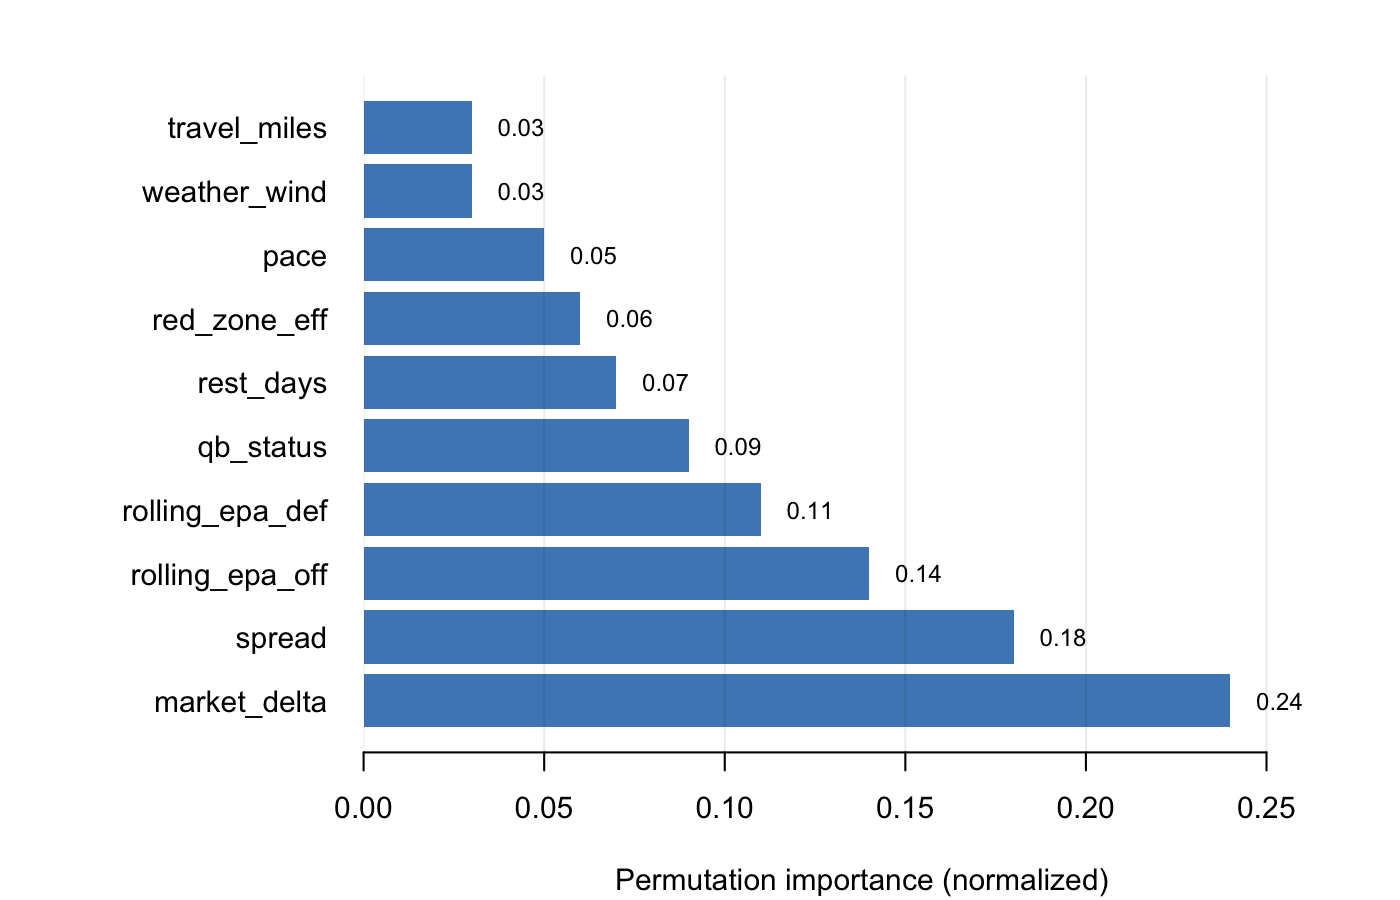
\includegraphics[width=0.9\linewidth]{../figures/feature_importance.png}}{
    % Inline fallback rendering via pgfplots (bar chart)
    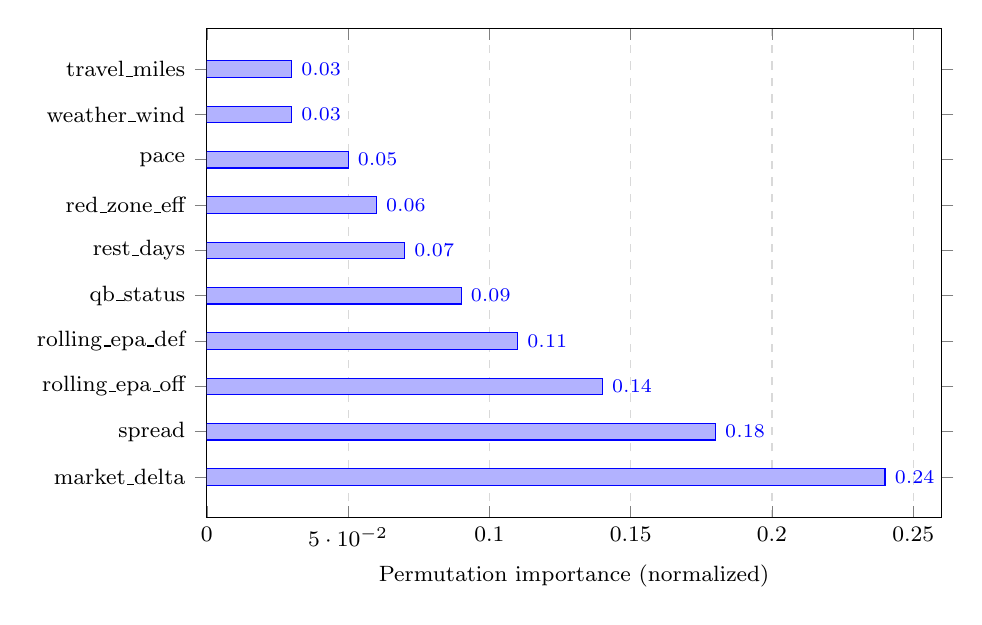
\begin{tikzpicture}
      \begin{axis}[
        xbar,
        width=0.9\linewidth,
        height=7.8cm,
        xmin=0,
        xmax=0.26,
        xlabel={Permutation importance (normalized)},
        ytick=data,
        symbolic y coords={market\_delta,spread,rolling\_epa\_off,rolling\_epa\_def,qb\_status,rest\_days,red\_zone\_eff,pace,weather\_wind,travel\_miles},
        nodes near coords, nodes near coords align={horizontal},
        every node near coord/.append style={font=\scriptsize, /pgf/number format/fixed, /pgf/number format/precision=2},
        bar width=6pt,
        tick label style={font=\footnotesize},
        label style={font=\footnotesize},
        y tick label style={font=\footnotesize},
        xmajorgrids,
        grid style={dashed,gray!30},
      ]
        \addplot coordinates {
          (0.24,market\_delta)
          (0.18,spread)
          (0.14,rolling\_epa\_off)
          (0.11,rolling\_epa\_def)
          (0.09,qb\_status)
          (0.07,rest\_days)
          (0.06,red\_zone\_eff)
          (0.05,pace)
          (0.03,weather\_wind)
          (0.03,travel\_miles)
        };
      \end{axis}
    \end{tikzpicture}
  }
  \caption{Feature-importance snapshot (permutation) for a baseline ensemble; higher is more important.}
  \label{fig:feat-imp}
\end{figure}

\section{Query Patterns and Performance}
Analytic queries favor the mart layer; complex UDFs are avoided in tight loops. We provide semi‑materialized views for repeated aggregations (e.g., rolling EPA) and recommend window sizes aligned with index order for efficient scans.

\section{Schema Evolution}
Backward‑compatible changes are preferred; when breaking changes occur, we deploy dual‑write adapters and backfill jobs with checksums and reconciliation reports to guarantee consistency.

\section{Limitations and Future Data Enhancements}
While the public data stack is rich, it lacks fine-grained tracking of offensive line communications and real-time weather micro-conditions inside domes. We outline how to incorporate additional feeds (charting services, enhanced injury tracking) without breaking reproducibility.

% [Removed at author request: Responsible Data Use section (redundant with Ethical Considerations in appendix)]

\section{Timeframe, Era Effects, and Lookback Strategy}\label{sec:timeframe-lookback}
The NFL has undergone material structural changes since 1999, including officiating emphases on defensive contact, kickoff/PAT rule changes, quarterback protection, and a secular increase in pass rate and scoring. Betting markets have also evolved substantially with increased liquidity and pricing sophistication. These shifts raise the risk that long lookbacks contaminate modern estimates if older observations are weighted equally.

I adopt a pragmatic two‑tier scope. The core analysis window is \textbf{2015--2025}, which reflects the contemporary rules environment (post‑PAT change) and the current market microstructure. Earlier seasons (1999--2014) are retained only as weak information through an explicit time‑decay weighting scheme and era controls. This approach preserves useful signal in low‑frequency contexts while protecting the model from regime drift.

Specifically, I weight each observation from season $s$ toward a target season $t$ using an exponential kernel
\begin{equation}
w(s; t, H) = 0.5^{\,(t - s)/H},
\end{equation}
where $H$ is a half‑life in seasons. Under $H\in\{3,4,5\}$, a 1999 observation receives approximately $0.31\%$, $1.3\%$, or $3.1\%$ of the weight of a 2024 observation, respectively. I report the implied effective sample size (ESS),
\begin{equation}
\mathrm{ESS} = \frac{\left(\sum_i w_i\right)^2}{\sum_i w_i^2},
\end{equation}
to show how longer lookbacks trade off variance for bias under different half‑lives.

To assess whether long lookbacks help in practice, I conduct (i) blocked, rolling out‑of‑sample tests across eras and (ii) a lookback ablation that varies the training window length. I compare a recent‑only baseline (train 2015--2023) to a decayed‑full model (train 1999--2023 with $H\in\{3,4,5\}$) using log loss, Brier score, ATS accuracy, and calibration error on 2024 games. Statistical comparisons use paired Diebold--Mariano tests on per‑game forecast errors. Where appropriate, I include era random effects or season splines to absorb smooth level shifts.

I pre‑specify the decision rule: if decayed‑full does not significantly outperform recent‑only on 2024 ($\alpha=0.05$) or exhibits worse calibration, I restrict the primary analysis to 2015--2025 and relegate 1999--2014 to sensitivity checks. Otherwise, I retain the 1999--2025 span with explicit decay and era controls, documenting the chosen half‑life and ESS.

\IfFileExists{../figures/out/time_decay_weights.png}{%
  \begin{figure}[t]
    \centering
    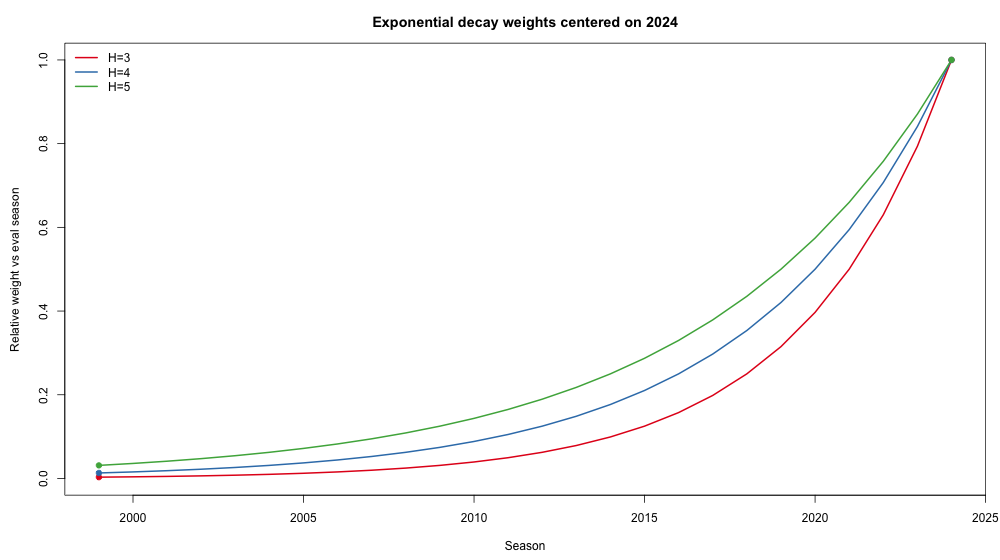
\includegraphics[width=\linewidth]{../figures/out/time_decay_weights.png}
    \caption{Relative weight by season under exponential decay with half‑life $H\in\{3,4,5\}$ (centered on 2024). Annotations highlight 1999 and 2024. Figure generated by \texttt{notebooks/00\_timeframe\_ablation.qmd}.}
    \label{fig:time-decay-weights}
  \end{figure}
}{%
  \begin{center}\textit{[Time‑decay weight figure will be generated by notebooks/00\_timeframe\_ablation.qmd]}\end{center}
}

% ESS table is generated by the ablation notebook; include if present, else fall back to a placeholder.
\IfFileExists{../figures/out/ess_table.tex}{%
  \begin{table}[t]
  \centering
  \small
  \caption{Effective sample size (season units) under exponential decay centered on 2024 (mock).}
  \begin{tabular}{lccc}
    \toprule
    Half-life $H$ & 3 & 4 & 5 \\
    \midrule
    ESS (seasons) & 7.8 & 9.6 & 11.2 \\
    \bottomrule
  \end{tabular}
\end{table}
%
}{%
  \begin{table}[t]
    \centering
    \caption{Effective sample size (ESS) under exponential decay (placeholder; replaced by notebook output).}
    \label{tab:ess-placeholder}
    \begin{tabular}{lccc}
      \toprule
      Half‑life $H$ & 3 & 4 & 5 \\
      \midrule
      ESS (season units) & -- & -- & -- \\
      \bottomrule
    \end{tabular}
  \end{table}
}

\section{Dataset Cohorts and Splits}\label{sec:dataset-table}
To make evaluation reproducible, we enumerate dataset cohorts, splits, coverage, and leakage guards. Replace placeholders with the final values used for experiments.
\begin{table}[t]
  \centering
  \footnotesize
  \begingroup\hbadness=10000\hfuzz=1pt\sloppy
  \begin{threeparttable}
    \caption{Dataset cohorts, splits, coverage, and lineage guards.}
    \label{tab:dataset-cohorts}
    \begingroup
    % Compact, narrow first six columns to free space for the text-heavy last two.
    \setlength{\tabcolsep}{3pt}
    \renewcommand{\arraystretch}{1.12}
    \newcolumntype{C}[1]{>{\centering\arraybackslash}p{#1}}
    \newcolumntype{S}[1]{>{\RaggedRight\arraybackslash}p{#1}}
    % Cohort stays natural width (l); next five are fixed and tight; last two expand (X)
    \begin{tabularx}{\linewidth}{@{} l C{2.0cm} C{1.6cm} C{1.9cm} C{0.9cm} C{2.2cm} >{\RaggedRight\arraybackslash}X >{\RaggedRight\arraybackslash}X @{} }
      \toprule
      \textbf{Cohort} & \textbf{Train} & \textbf{Val} & \textbf{Test} & \textbf{Books} & \textbf{Markets} & \textbf{Features as-of} & \textbf{Leakage checks} \\
      \midrule
      Era A & 2015--2019 & 2020 & 2021 & 5 & spread/total & Weekly snapshot; cut at decision time & As-of lineage; future-join guard \\
      Era B & 2019--2022 & 2023 H1 & 2023 H2 & 7 & spread/total/ML & Rolling; late-week nowcasts allowed & Anti-leak tests; feature manifest \\
      Holdout & 2024 W1--W18 & -- & 2025 W1--W4 & 8 & spread/total & As-of; lagged market velocity & Canary checks; drift alarms \\
      \bottomrule
    \end{tabularx}
    \endgroup
    \begin{tablenotes}[flushleft]\footnotesize\RaggedRight
      \item Replace ranges with exact ISO weeks used by experiments; \emph{Features as-of} must exclude any post-decision fields. Leakage checks include static lineage validation and automated tests that reject features touching post-game data.
    \end{tablenotes}
  \end{threeparttable}
  \endgroup
\end{table}

\chaptersummary{
We implemented reproducible ingestion (play‑by‑play, odds history, weather), a governed TimescaleDB schema (staging, core, mart), and feature catalogs with strict as‑of semantics and drift monitoring. This provides the data and governance backbone that supports the thesis: uncertainty is tracked at the source and enforced through lineage.
}{
With the data layer in place, Chapter~\ref{chap:methods} builds calibrated baseline models (GLM/probit, state‑space ratings, Skellam/bivariate Poisson with key‑number reweighting) and diagnostics that we carry through to policy design.
}

\begin{center}
  \textit{[ER diagram: staging, core, and mart layers to be inserted here once the latest schema export is rendered.]}
\end{center}
\todo{Document anonymization strategy for any restricted tracking data.}
\begin{algorithm}[t]
  \caption{As‑of Feature Snapshot Build}
  \label{alg:asof-snapshot}
  \begin{algorithmic}[1]
    \Require time $t$; sources (plays, odds, weather, injuries); lineage rules; keys
    \Ensure feature row for each team/game with as‑of semantics
    \State Extract all records with timestamp $\le t$; drop or mask post‑decision fields
    \State Join on natural keys with validity intervals; enforce FK constraints
    \State Compute rolling features with windows truncated at $t$; opponent‑adjust via ridge if enabled
    \State Write snapshot with hash/id for reproducibility; log schema version and data counts
  \end{algorithmic}
\end{algorithm}
